\documentclass[10pt,
%showpacs,
amsmath,amssymb,
aps,prd,nofootinbib,eqsecnum,a4paper]{revtex4}
\usepackage{graphicx,epsf}
\usepackage{float}
\usepackage{wrapfig}
%
\usepackage{xcolor}
\usepackage[colorlinks = true,
            linkcolor = blue,
            urlcolor  = blue,
            citecolor = blue,
            anchorcolor = blue]{hyperref}
%
\topmargin-10mm
%
%
\def\be{\begin{equation}}
\def\ee{\end{equation}}
%
\def\bea{\begin{eqnarray}}
\def\eea{\end{eqnarray}}
%
\def\p{\partial}
\def\n{\nabla}
\def\dkk{\p_k\p^k}
\def\sh{{\sigma}}
\def\L{{\pounds}}

\usepackage{framed}


\usepackage{float}

\newcommand{\CC}{C\nolinebreak\hspace{-.05em}\raisebox{.4ex}{\tiny\bf +}\nolinebreak\hspace{-.10em}\raisebox{.4ex}{\tiny\bf +}}
\def\CC{{C\nolinebreak[4]\hspace{-.05em}\raisebox{.4ex}{\tiny\bf ++}}}
\def\S{ }
\begin{document}


\title{PyTransport: A Python package for the calculation of inflationary correlation functions}
\author{David J. Mulryne}
\affiliation{Astronomy Unit, School of Physics and Astronomy,
Queen Mary University of London, Mile End Road, London, E1 4NS, UK}
\email[]{d.mulryne@qmul.ac.uk}

\date{\today}

\begin{abstract}

\noindent PyTransport constitutes a straightforward code written in \CC \S  together 
with easy to use Python scripts which automatically edit, compile and run the \CC \S code as a 
Python module. It has been written for Unix-like systems (OS X and Linux) using Python 2.7.
Among other things, the module employs the transport approach to inflationary cosmology to calculate 
the tree-level power-spectrum and bispectrum of user specified models of multi-field inflation, 
accounting for all tree-level sub and super-horizon effects.
The transport method we utilise means 
only coupled differential equations need to be solved, and the implementation presented here 
combines the speed of \CC \S  with the functionality and convenience of Python. At present the code 
is restricted to canonical models.
This document details the code and illustrates how to use it with a worked example.


\end{abstract}

\maketitle

%%%%%%%%%%%%%%%%%%%%%%%%%%%%%%%%%%%%%%%%%%%%%%%%%%%%%%%%%%%%%%%%%%%%%%

%%%%%%%%%%%%%%%%%%%%%%%%%%%%%%%%%%%%%%%%%%%%%%%%%%%%%%%%%%%%%%%%%%%%%%

%%%%%%%%%%%%%%%%%%%%%%%%%%%%%%%%%%%%%%%%%%%%%%%%%%%%%%%%%%%%%%%%%%%%%%


%\begin{wrapfigure}{L}{9cm}
\begin{figure}[H]
\centering
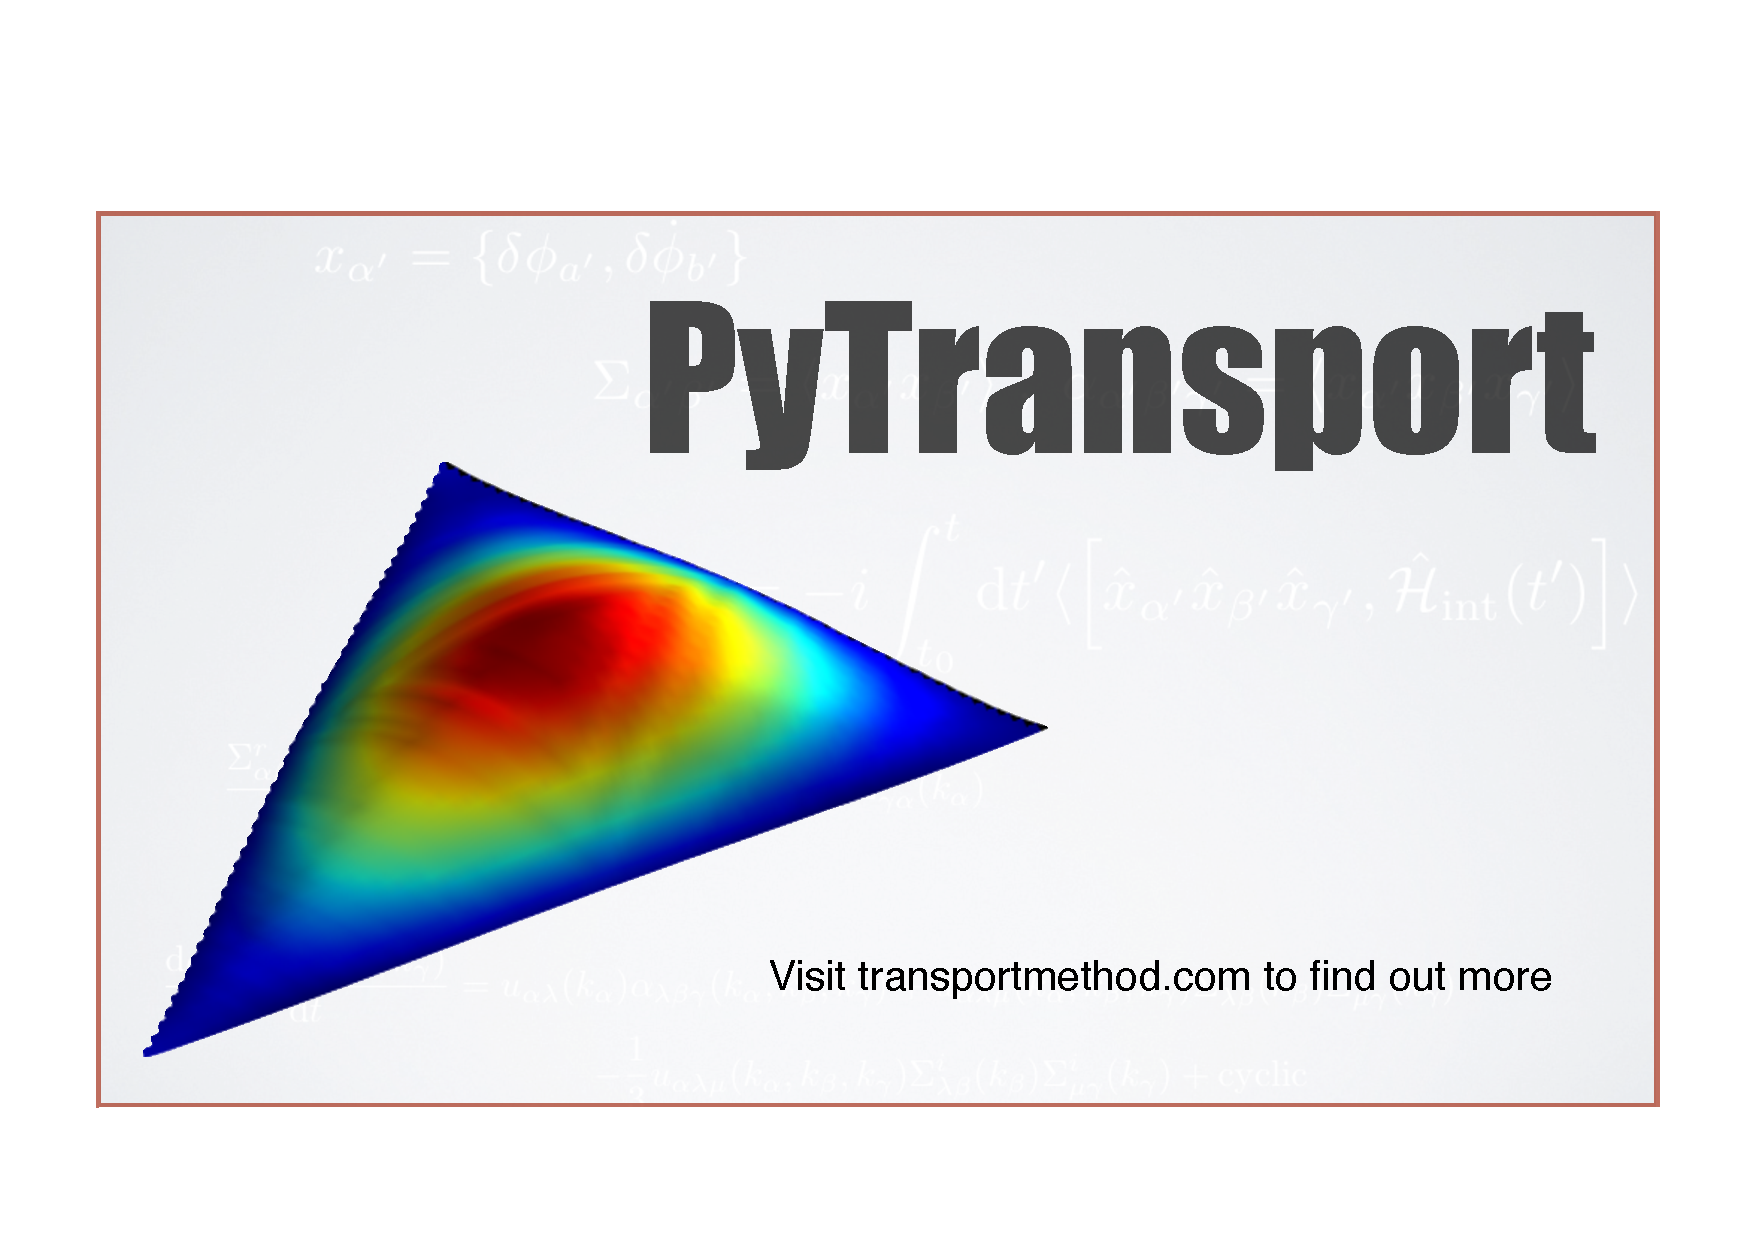
\includegraphics[width=11cm]{PyTransLogo}
\end{figure}
%\end{wrapfigure}


\section{Introduction}

\begin{framed}
{\bf \noindent PyTransport is distributed under a GNU GPL licence. If you use PyTransport you are kindly asked to cite Ref.~\cite{xxx}  as well as the archive version of this user guide in any resulting works. }
\end{framed}

The main purpose of this document is to teach those interested how to use, and if so desired adapt, 
the PyTransport package. 
The philosophy behind this implementation of the transport method is simplicity and ease of use. 
Python was selected as the 
language though which to interact with the code because it enables rapid scripting and provides a flexible 
and powerful platform on which to study inflationary cosmology. In particular, it has many readily available tools and packages for analysis and visualisation, and for tasks such as parallelisation  (using for example Mpi4Py).  

As an interpreted language, however, Python can be slow for some tasks. This is circumvented here by 
using \CC \S  code, 
which is compiled into a Python module, to perform numerically intensive tasks with the result that the speed 
of the package is nearly indistinguishable from pure \CC. The \CC \S  code itself is kept as simple and 
clean as possible, and therefore can easily be edited if required. PyTransport has been developed on 
Unix-like systems 
using Python 2.7. The author uses OS X  and the Enthought Canopy environment. used by the 
author, and with additional testing performed on a Linux system also with Python 2.7. 
It seems likely it could easily be adapted to Windows systems, but this has not yet been attempted,
 and there shouldn't be significant issues moving to Python 3.

The transport approach the code employs 
can be seen as the differential version of the integral expressions of the In-In formalism. It 
is helpful numerically because it provides a set of ordinary differential equations for the correlation functions  
of inflationary perturbations. The code then solves these equations from deep inside the horizon until some desired time 
after horizon crossing using a standard variable step size ordinary differential equation (ODE) 
routine with error control. Such off the shelf 
routines are extremely well tested, and provide
an easy way to change the required accuracy. This is helpful in order to check convergence of the numerical 
solutions, or to respond to needs of models with very fine features. 
Details of the transport method itself that the code is based on can be found in the recent paper \cite{xxx}. We 
highly recommend reading this guide in combination with that paper.
 
The code is intended to be a reusable resource for inflationary cosmology. It enables users to quickly create a 
complied Python module(s) for any given model(s) of multi-field inflation. The module contains a number of
functions that can be called from Python and that perform tasks such as calculating the background evolution 
of the cosmology, and the two and three point function's evolution. We provide a number of further functions written in 
Python which perform common tasks such as calculating the power spectrum or bispectrum over a range of scales, 
but the true power of the approach is that users can rapidly write their own scripts, or adapt ours, to suit their own needs. 

First we give some brief background and motivation for the code, much more can be found in Ref.~\cite{xxx}, 
before giving an overview of its structure and how 
it can be set up. In the appendices we give some more detail about the structure of the underlying \CC \S code,  
give full details of all the functions the complied module provides, and all the functions provided by 
Python scripts which accomplish common tasks. The best way to learn how to use the package, however, is 
by example. We present an extended example below spread between the ``Getting going"  and ``Examples" sections, 
complete with screen shots of the code in use. 
Other examples which come with the distribution are discussed in the ``Examples" section.
Throughout, familiarity with Python and to some extent \CC \S  is assumed, though in reality users 
can just probably get a long way by looking at the examples and modifying to their needs. 



Finally, we would also like to refer readers to the complementary package developed 
in tandem with the work in Ref.~\cite{xxx} and with PyTransport: CppTransport \cite{xxx2}. This is a platform for inflationary 
cosmology developed fully in \CC. In comparison with PyTransport it  has 
more external dependancies (in the sense that the dependancies of PyTransport are mainly 
Python modules), but provides more sophisticated parallelisation and data management capabilities. 
In limited testing it is also found to be marginally faster.
For users with modest aims in terms of CPU hours and data generation, however, it is likely to have a higher 
overhead 
in getting started, but may well be very beneficial for intensive users. PyTransport 
is intended to be more lightweight with users encouraged to utilise the power of Python in combination 
with PyTransport to achieve their specific aims and data management needs


\section{Background} 

Calculations of the correlation functions of perturbations produced by inflation 
are now extremely mature.
In the single field context, the In-In formalism is routinely used to calculate the equal time correlation 
functions of the 
curvature perturbation, $\zeta$, as wavelengths cross the cosmological horizon 
\cite{Maldacena:2002vr, Seery:2005wm, Chen:2006nt,Elliston:2012ab}, where they become 
constant \cite{Rigopoulos:2003ak,Lyth:2004gb}. 
For many models this calculation can be accurately performed 
analytically, while for others, such as models with features, 
a numerical implementation is required \cite{Chen:2006xjb,Chen:2008wn,Hazra:2012yn,Funakoshi:2012ms}. 
If additional fields are added, the problem becomes even more complex. $\zeta$ is no longer 
necessarily conserved after horizon crossing, and the evolution of all 
isocurvature modes needs to be accounted for   
from initial vacuum sate until such time as the system becomes adiabatic, or until the time at which we wish to know the statistics  (see for example Ref.~\cite{Elliston:2011dr} 
for a discussion of adiabaticity). While analytic progress can be made in some circumstances 
using the In-In formalism and/or so called ``super-horizon" techniques such as the $\delta N$ formalism, 
in general for multiple field models numerical techniques become even more important. 

The code documented here accounts for all tree-level effects present in multi-field inflation. This includes  
the super-horizon evolution of $\zeta$, which 
can occur in models with multiple light  
fields, as well as the effect of features in the multidimensional potential, and the effect of 
quasi-light or heavy fields orthogonal to the inflaton 
(which are important if the inflationary trajectory is not straight).
As discussed above the code utilises the transport approach to inflationary correlation functions 
\cite{Mulryne:2009kh,Mulryne:2010rp,Dias:2011xy,Anderson:2012em,Seery:2012vj, Mulryne:2013uka}. This approach 
can be viewed as a differential version of the integral expressions of the In-In formalism, 
and evolves correlations of inflationary perturbations from their vacuum state on 
sub-horizon scales until we wish to evaluate the statistics. 
We note for clarity, that in its original form the ``moment transport'' method was restricted 
to super-horizon scales, but it was later shown how it could be extended to include sub-horizon scales 
in Ref.~\cite{Mulryne:2013uka}. A recent paper studies this extension further and develops it into a working 
algorithm \cite{xxx} with many additional details provided. The present document details 
the code PyTransport which implements that algorithm.

The objects of primary interest for users to calculate in inflationary cosmology are the background inflationary 
fields, $\phi_i(t)$, and associated velocities (the rate at which the fields change with cosmic time), $\dot \phi_i(t)$,
as well as the number of e-folds which the evolution gives rise to, the correlations of the perturbations in these fields, 
and correlations of other perturbative quantities.  Here we have used the label $i$ 
to run over the number of fields present. 
The code solves the equations of motion for the background cosmology and 
the correlations of the field and field velocity perturbations 
defined on flat hyper-surfaces. Ultimately the quantities 
probably of most interest for observations are the power spectrum and bispectrum 
of the curvature perturbation $\zeta$. 
Defining the array ${\mathbf X} = \{{\mathbf \delta \phi}, \mathbf {\delta \dot \phi} \}$, where 
the components are labelled $X^a$ and $a$ now runs over the total number of fields and field derivatives, 
we recall the following definitions for later clarity:
\begin{eqnarray}
\langle \zeta(\mathbf{k_1}) \zeta(\mathbf{k_2})  \rangle &=& (2\pi)^3 \delta(\mathbf{k}_1 + \mathbf{k}_2 )
        P_\zeta(k_1) \,, \\
\langle X^a(\mathbf{k_1}) X^b(\mathbf{k_2})  \rangle &=& (2\pi)^3 \delta(\mathbf{k}_1 + \mathbf{k}_2 )
        \Sigma^{ab}(k_1) \,, \\
\langle \zeta(\mathbf{k_1}) \zeta(\mathbf{k_2}) \zeta(\mathbf{k_3}) \rangle &=& (2\pi)^3 \delta(\mathbf{k}_1 + \mathbf{k}_2 + \mathbf{k}_3)
        B_\zeta(k_1, k_2, k_3) \,, \\
\langle X^a(\mathbf{k_1}) X^b(\mathbf{k_2}) X^c(\mathbf{k_3}) \rangle &=& (2\pi)^3 \delta(\mathbf{k}_1 + \mathbf{k}_2 + \mathbf{k}_3)
        B^{abc}(k_1, k_2, k_3) \,, 
\end{eqnarray}
where $P_\zeta$ and $B_\zeta$ are power spectrum and bispectrum of $\zeta$ respectively, 
and $\Sigma$ and $B$ are 
the equivalent functions for the correlations and cross correlations in field space. 
$\Sigma$ and $B$ together with the background 
values of the fields and field velocities are the objects directly evolved by the code using the equations 
detailed in section~5 of Ref.~\cite{xxx} with 
initial conditions 
detailed in section~6 of Ref.~\cite{xxx}\footnote{Internally the code internally rescales 
the field velocity perturbation $\delta \dot \phi$ for 
performance reasons, as well as internally rescaling the wavenumbers involved, but the rescaling is reversed before 
outputing results -- this is discussed further in the appexdix 1.}. As 
discussed in that paper, $B$ and $\Sigma$ can then 
readily be converted to give $P_\zeta$ and $B_\zeta$ through the use of the ``$N$" tensors with components $N_a$ and $N_{ab}$, 
described in section~7 of Ref~\cite{xxx} (see also \cite{Dias:2014msa}). 
The equations of motions for the correlations 
are given in Eqs.~(5.5) and (5.16) of  Ref.~\cite{xxx}, the initial conditions in Eqs.~(6.2) and (6.7),
and the conversion to $\zeta$ in 
Eq.~(7.4) .


It is worth briefly commenting on how our code compares with existing ones. A number of publicly available 
codes exist to calculate the power spectrum from canonical multi-field inflation. 
For example Pyflation \cite{Huston:2011fr} and 
MultiModeCode \cite{Price:2014xpa} employ a method originally used by Salopek and Bond \cite{Salopek:1988qh}
in which the mode functions of the QFT of inflationary perturbations are evolved. These codes are 
in written Python\footnote{Pyflation also makes sure of C code for speed through the use of Cython} and Fortran respectively.
Moreover, a Mathematica code which implements the transport method for curved field space 
metric models, but is restricted to the power-spectrum, is also available
\cite{Dias:2015rca}. At the level of the three point function a number of authors have undertaken 
numerical work utilising 
directly the In-In formalism for example in Refs.~\cite{Chen:2006xjb,Chen:2008wn, Hazra:2012yn,Funakoshi:2012ms,Horner:2013sea}. 
The only publicly released code we are aware of, however, is BINGO \cite{Hazra:2012yn} which is restricted to single field models. 
No general multi-field codes have been undertaken until now.

An further advantage of PyTransport (and CppTransport) over previous codes is that it leaves
little for the user to calculate analytically. 
It needs the user 
to provide only the inflationary potential. Then all the derivatives are automatically calculated using 
symbolic Python (SymPy) and written automatically into the \CC \S  code which is then compiled. 
Compared to Fortran or pure \CC \S  
implementations, PyTransport 
has the advantage of easy access to the extensive and easy to use modules available to 
Python, and compared to a pure Python or Mathematica implementations we have the advantage of speed.


\section{ Code overview} 

\noindent  The code structure should become familiar though the extended example we provide, but here we give a brief summary. 

The code is distributed in a folder called {\it TransportDist/} , which also contains a copy of this document (possibly updated compared with the arXiv version) in the 
{\it TransportDist/docs/} folder. The base code for PyTransport is written in \CC \S , and has a simple object orientated structure. This code can be found 
in the {\it TransportDist/PyTransport/CppTrans} folder and we provide a few more details about its structure 
and functionality in  Appendix 1. 
The \CC \S code is deliberately as simple as possible to ensure transparency 
and adaptability. The idea of the PyTransport package as a 
whole, is that once a potential is provided by the user, 
the \CC \S  code is automatically edited and complied into a Python module by supporting 
Python functions (called from the {\it TransportDist/PyTransport/PyTransSetup.py} file), 
which means a lot of work is done for the user.  
The end result is a Python module consisting of a set of Python functions for a specific inflationary potential, called the 
PyTrans*** module. 
The functions of this module provide key routines for inflationary cosmology (including calculating the correlations 
up to the bispectrum). The asterisks *** indicates we can label the module with a tag telling us what potential it 
corresponds to if we wish, and we can 
therefore install multiple modules if we want to work with many potentials simultaneously. The 
key functions available to these modules 
are defined in the file {\it TransportDist/PyTransport/PyTrans/PyTrans.cpp} (which is a \CC \S  file defining the
 Python module), these function are detailed in Appendix~3.
The scripts  that edit the \CC \S code and compile the module are discussed further below in the setup section, 
and by default they place the compiled module in the local folder 
{\it TransportDist/PyTransport/PyTrans/lib/python/} to avoid access issues if, for example, you do not have root privileges. 
Other useful Python functions that perform common tasks, such as producing a power spectrum by looping 
over call is to the compiled module, can be 
found in {\it TransportDist/PyTransport/PyTransScripts.py}, and we describe them below, and detailed in full in Apendix~4. 
Python 
treats functions written in Python inside a file such as {\it PyTransScripts.py} and {\it PyTransSetup.py}, 
in the same way as a compiled module. 
So there are effectively {\bf three modules within PyTransport }, 
one to setup a compiled module for the potential we want to study ({\bf PyTransSetup}), the compiled module itself ({\bf PyTrans}) 
(or multiple complied modules labeled with different tags), and a 
module with various functions automating common tasks that 
use the functions of the compiled module ({\bf PyTransScripts}). 
Also in the {\it PyTransportDist/} folder is an example folder {\it PyTransportDist/Examples} 
containing the examples discussed below.


We note that all the \CC \S  code is written by the transport team except for an included Runge-Kutta-Fehlberg (rkf45)
integrator routine written by John Burkardt and distributed under a GNU LGPL license detailed \href{https://people.sc.fsu.edu/~jburkardt/f_src/rkf45/rkf45.html}{here}\footnote{$\rm https://people.sc.fsu.edu/~jburkardt/f_src/rkf45/rkf45.html$}.  We choose this lightweight integrator over other options, such as using integrators included with 
the BOOST library, in order that it could easily be included with the distribution with no external dependancies being introduced. 
In our (limited) testing it functions well for all the models we have looked at.
There are no dependancies external to the folders provided except for a working Python 
installation (with appropriate packages downloaded), and a \CC \S compiler -- this is deliberate to make 
using the code as easy as possible to use.
An MPI installation such as openMPI is also needed if the module is required to be 
used across multiple cores. 

\section{Setup}
\label{Setup}

\subsection {Prerequisites} 

\noindent  So what is needed? The idea is as little as possible beyond Python:

\vspace{0.2cm}
\noindent {\bf Python:}  A working Python installation is needed, we use Python 2.7. 
For convenience the author recommends downloading a complete Python distribution, for  
  example Enthought Canopy, Pythonxy, Continuum Anaconda, or similar distribution, which come with all 
  the core Python packages used by this code. Enthought Canopy is used by the author. 
  They also come with interactive environments which can be convenient for development purposes.
  Python packages currently used by PyTransport or by provided examples include Numpy, Matplotlib, SciPy, SymPy, Distutils, Math and Sys, 
  as standard, and Mpi4Py and Mayavi are used 
  for MPI and 3D bispsectra plots respectively. Of these only Mpi4Py and Mayavi may 
  need to be downloaded separately from the distributions mentioned. The easiest way to install a package 
  such as Mpi4Py is to type 
 ``pip install Mpi4Py" in the terminal. Mayavi can also be installed in this way, or if using Canopy 
 then Canopy's own package manager is an even easier way to do this. If you do not have root 
 privileges then ``sudo" must be added before ``pip". There are many 
 easily found resources on the internet to help with such installations if there is a system 
 specific snag. Note that you should not attempt to install Mpi4Py with installing MPI first (which we deal with next).

\vspace{0.2cm}
\noindent {\bf MPI:}
As computing the bispectrum can be computationally expensive, distributed computing can be helpful 
(even across the multiple cores of modern PCs). 
In some of the scripts in the 
{\it PyTransScripts} module,  
we use the Mpi4Py module to implement this. Mpi4Py needs a working MPI installation such as 
openMPI installed on your 
computer. Note that Mpi4py or openMPI are not needed for 
PyTransport in general, and if you do not have these installed you simply  
cannot run the scripts that use MPI, but can run the code in serial instead. A nice guide to installing openMPI is 
at this \href{https://wiki.helsinki.fi/display/HUGG/Open+MPI+install+on+Mac+OS+X}{link}\footnote{https://wiki.helsinki.fi/display/HUGG/Open+MPI+install+on+Mac+OS+X}.

\vspace{0.2cm}
\noindent {\bf \CC \S  complier}
Python needs to be able to find a \CC \S  complier in order to compile the PyTrans module(s). This is bundled with most 
Linux distributions. If not present on a Mac system, downloading Xcode from the app store is the easiest way to 
install one.

\subsection{Getting going}

\noindent  Once you have Python running and a \CC \S compiler, to get started take the {\it PyTransport/} folder from the 
{\it TransportDist/} folder and place it 
anywhere convenient in your computer's file system. It is essential that you don't change 
the structure of the sub-directories within {\it PyTransport/} , but you can place this folder wherever you want.  
That's more or less all you have to do.
You can do this by copying the entire folder {\it TransportDist/} (which 
also contains examples and this guide) to a convenient location, but equally well you could run examples from 
anywhere else on your computer. In each example, we will see one needs to add the path of  
the {\it PyTransport/} folder to the paths which Python includes when looking for code, so that Python can 
find the setup file 
{\it PyTransSetup.py} (or this could be done permanently).

Now you can get started, no other installation is required which is not handled for you by provided 
Python scripts.

Lets say you want to analyse the inflationary model defined by the potential
\be
V=\frac{1}{2} m^2_{\phi} \phi^2 + \frac{1}{2} m^2_{\chi} \chi^2\,.
\ee
The first step is to create (by compiling the \CC \S  code) a Python module for this potential. This is achieved by writing 
the potential in a Python file in SymPy (symbolic Python notation) and calling the 
appropriate functions from the { PyTransSetup module}. First define two SymPy 
arrays one for the fields and the other for parameters which 
define the model (and whose values you might wish to change). These have length nF and nP respectively. 
Then define the symbolic potential $V$ using these arrays. The potential must be written into the 
\CC \S  code by calling the function {\it potential(V,nF,NP)'}  which is in the file {\it PyTransSetup.py}.  
Then the function {\it compile()} or {\it compileName(Quad)} 
(where ``Quad'' can be replaced by any name the user likes (the *** from above)) also in 
{\it PyTransSetup.py} is called to create the Python module. The difference between the two compile 
functions is that one creates a module called { PyTrans}, which would simply be  written over if a user moved on 
to a different potential, and used compile again, while the second gives the module a tag and creates (in this case) 
the module PyTransQuad. Multiple modules for different potentials with different names can therefore be created and 
used simultaneously. Below is a screen shot of the procedure just described with copious comments which should 
make the procedure clear:

\begin{figure}[H]
\centering
\includegraphics[width=18cm]{shot1c}
\end{figure}

This example is contained in the {\it DoubleQuad/} folder in the {\it Examples/} folder which accompanies the code, with this script in the file {\it DQuadSetup.py} file. In this script 
we have used three functions from the PyTransSetup module, the two mentioned above, and {\it tols(rel, abs)}, 
which sets 
the relative and absolute tolerances of the ode integrator (note we need to reinstall the compiled 
module if we wish to alter these tolerances). Appendix 1 contains a summary of all the functions 
available in the setup module.

We can now use the complied Python module. To do so we need to point Python to the path of the new module (and 
the scripts module). This can be done for us by calling the function in the setup module {\it pathSet()}. We recommend using the {\it PyTransQuad} module in a separate file from the one used to set it up, and if working in an integrated development environment to restart the Python kernel (this is to ensure the most recent version is always imported). Below is a screen shot of the start of a file in which we use the module set up in the previous paragraph. First 
to simply calculate the value of the potential and the derivative of the potential for particular field values and parameters,
and use these to set up an array containing field values and the associated fields velocity (using the slow roll
equation):


\begin{figure}[H]
\centering
\includegraphics[width=18cm]{shot2}
\end{figure}

This screen shot is of the start of the file {\it Examples/DoubleQuad/SimpleExample.py}. Of course we will usually want 
to use the module for more sophisticated tasks. Appendix 4 contains a summary 
of all the functions  available within the { PyTrans***} module. We will see the use of a number of the more sophisticated functions in the 
Examples section.

\section{Examples}
\label{Examples}

\subsection{Double quadratic}

First lets continue with the double quadratic example using more of the functions 
available from the compiled module. In the screen shot below we use the background evolution 
function to calculate a fidicual background trajectory in field space using the array we set up in the last 
part of the example as initial conditions. The function used in the {\it PyTrans.backEvolve} function. 
The output is plotted shown in Fig.~\ref{double1}. Then we run the two point evolution function to calculate evolution 
of $\Sigma$ and the power spectrum of $\zeta$ for a $k$ mode which crossed the horizon 
10 e-folds into this fiducial run using the {\it PyTrans.sigEvolve} function. 
We plot the correlations and cross correlations of the fields in Fig.~\ref{double2}. 
We repeat for a neighbouring $k$ to give us a crude estimate of $n_s$ the spectral index. 
Finally, we run the three point evolution function for a set of three $k$s to calculate the evolution of 
the three point function in field space, and the bispectrum of $\zeta$ using the {\it PyTrans.alphaEvolve} function. 
We 
plot the three-point correlations and cross correlations of the fields in Fig.~\ref{double2} for the
and also plot the evolution of the reduced bispectrum, denoted $f_{\rm NL}$. In the plots it can clearly be 
seen that the heavier field drops out of the dynamics at around 40 e-folds. At this 
point the system becomes adiabatic and $\zeta$ and its statistics become constant.
A screen shot of the code which does all this from the {\it SimpleExample.py} file is below:
\begin{figure}[H]
\centering
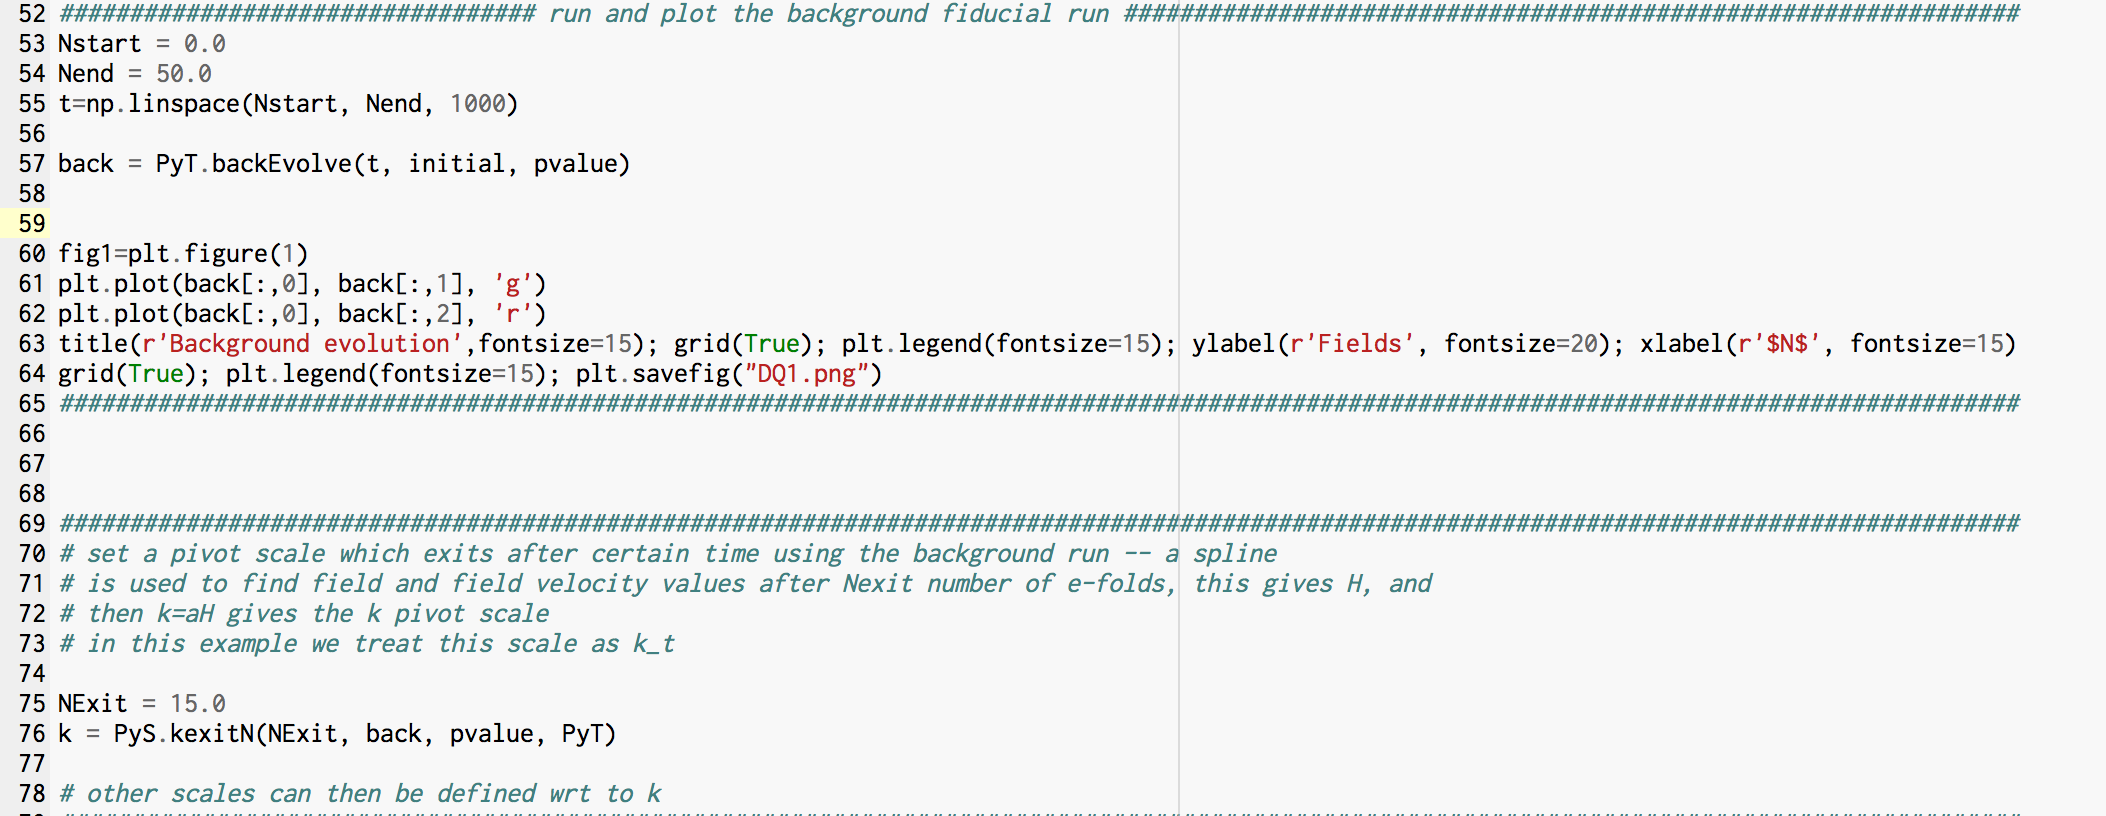
\includegraphics[width=17.2cm]{Shot3}
\end{figure}
\begin{figure}[H]
\centering
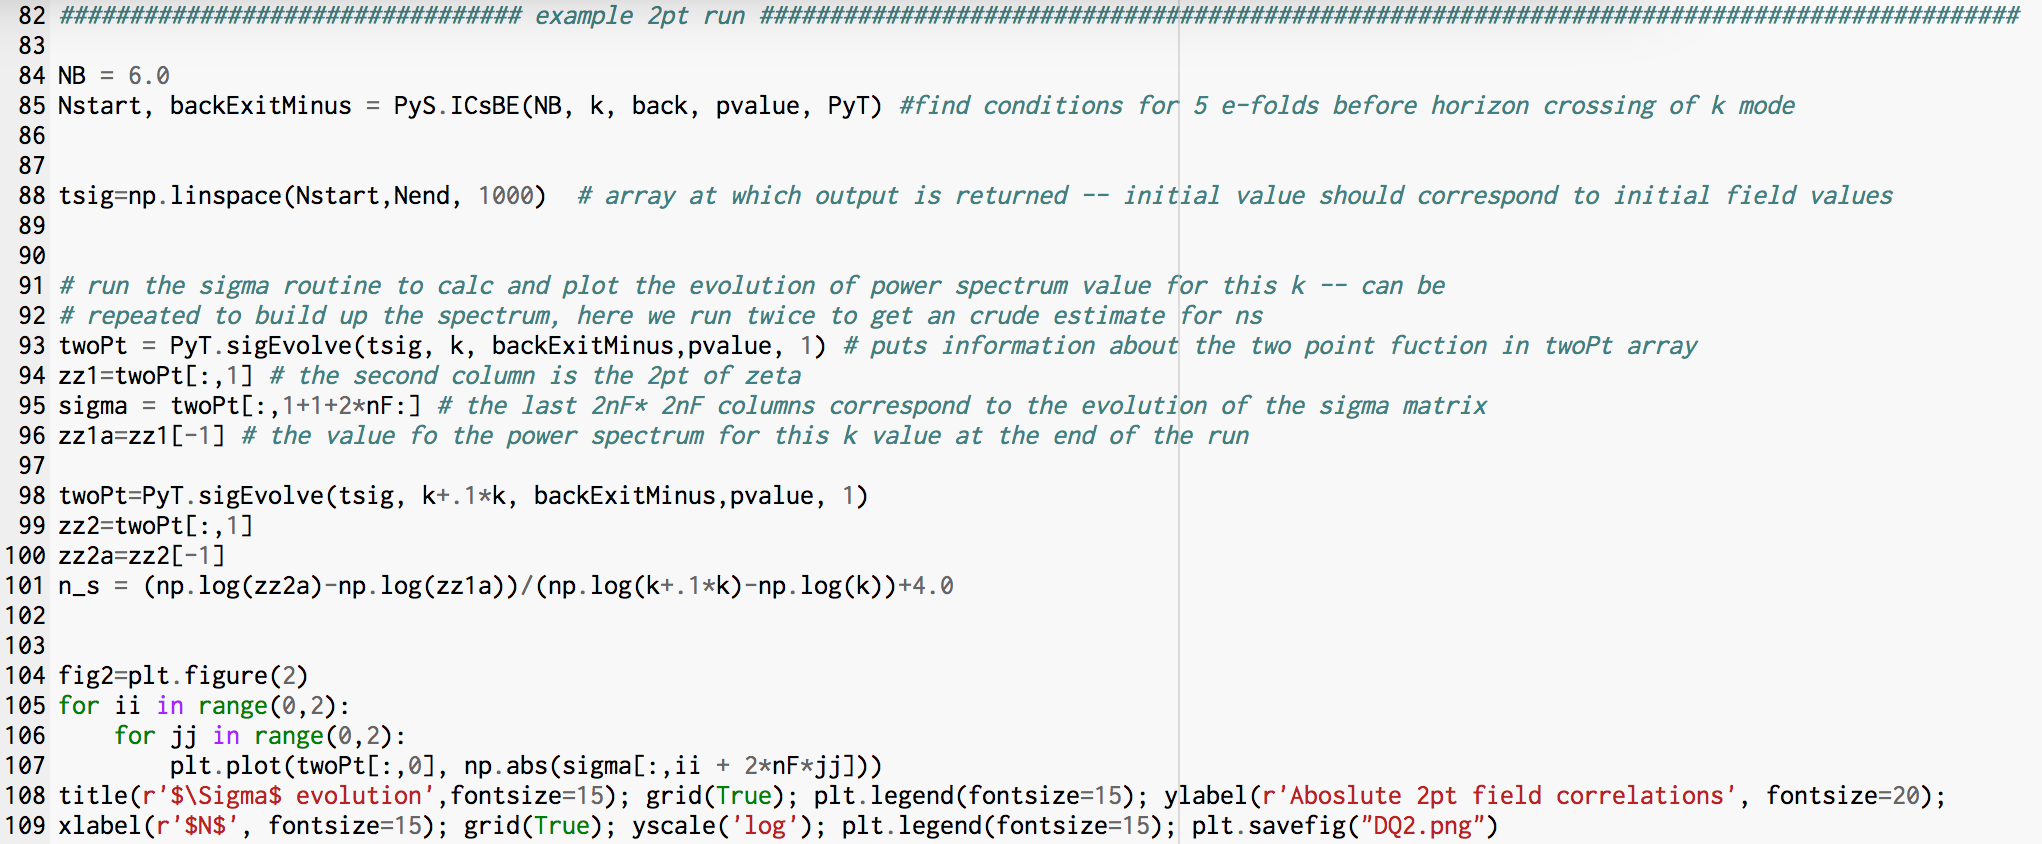
\includegraphics[width=17.2cm]{Shot4}
\end{figure}
\begin{figure}[H]
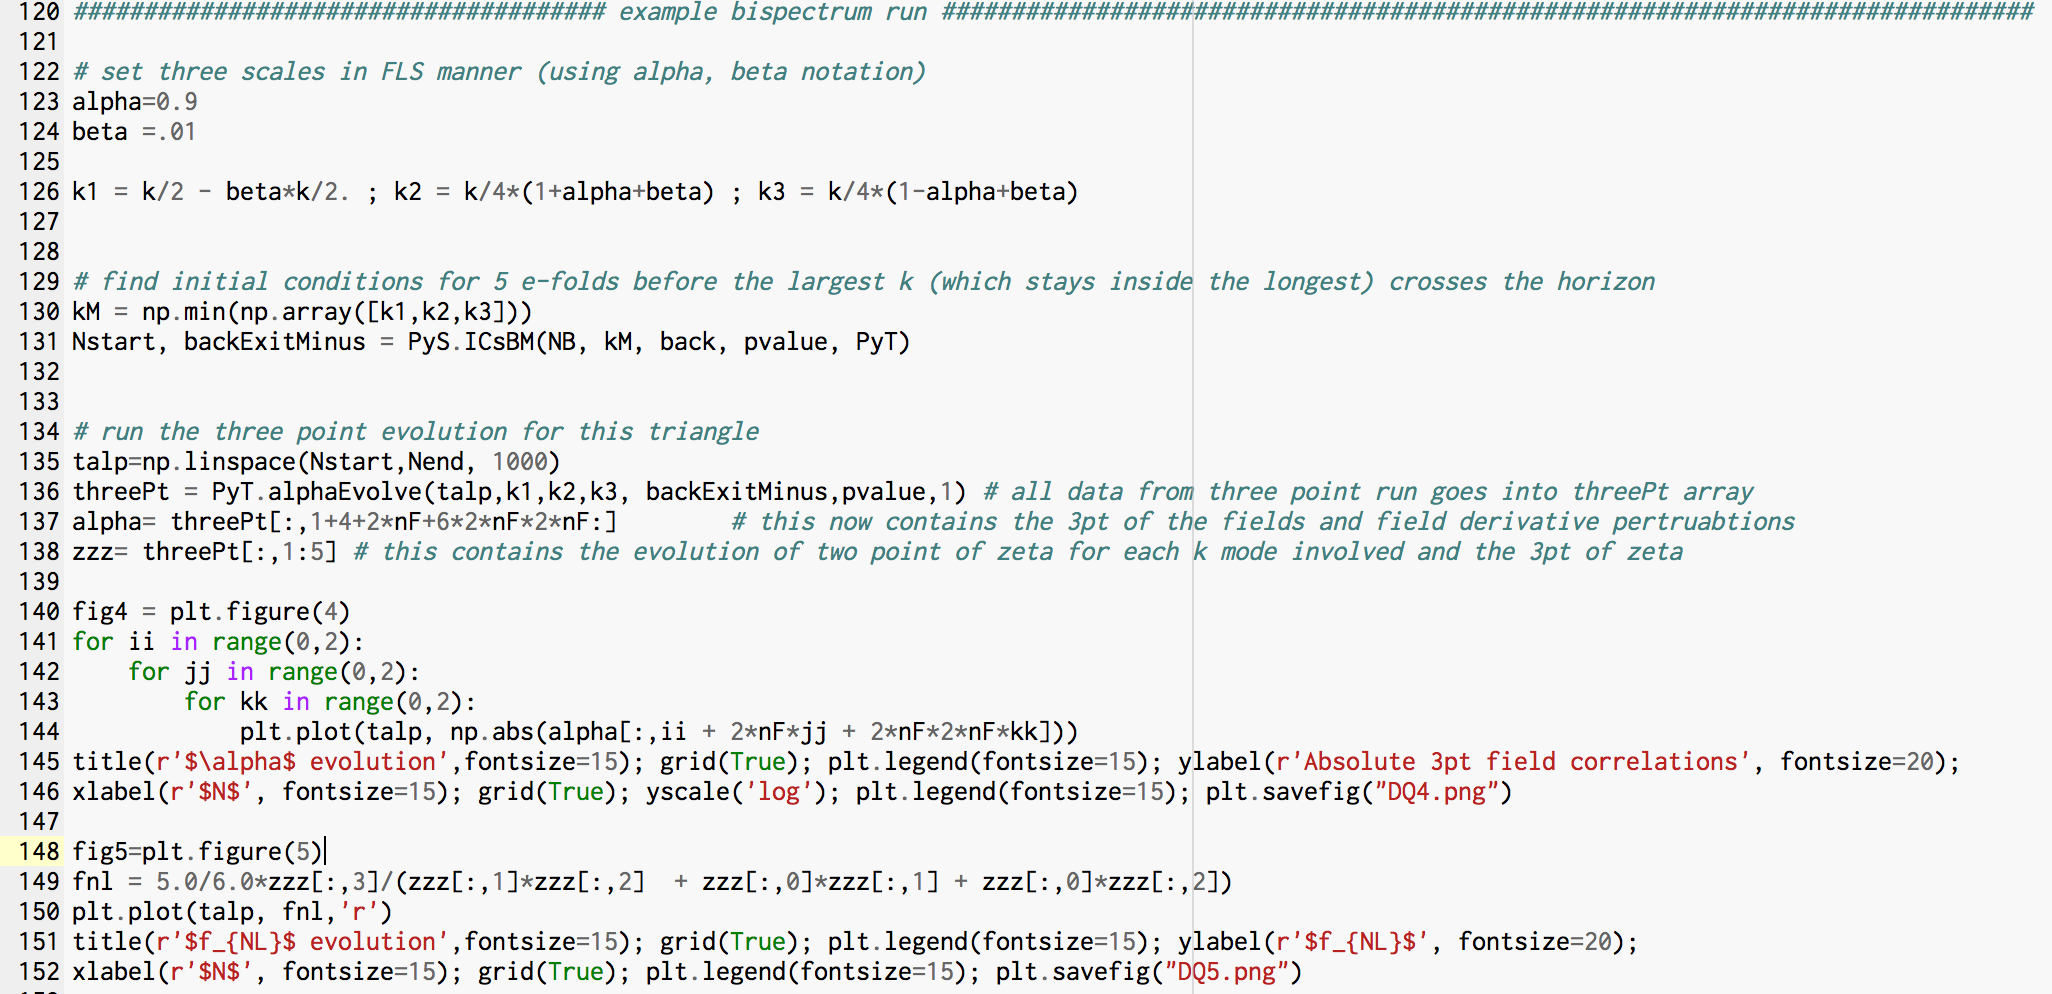
\includegraphics[width=17cm]{Shot5}
\end{figure}



\begin{figure}
\centering
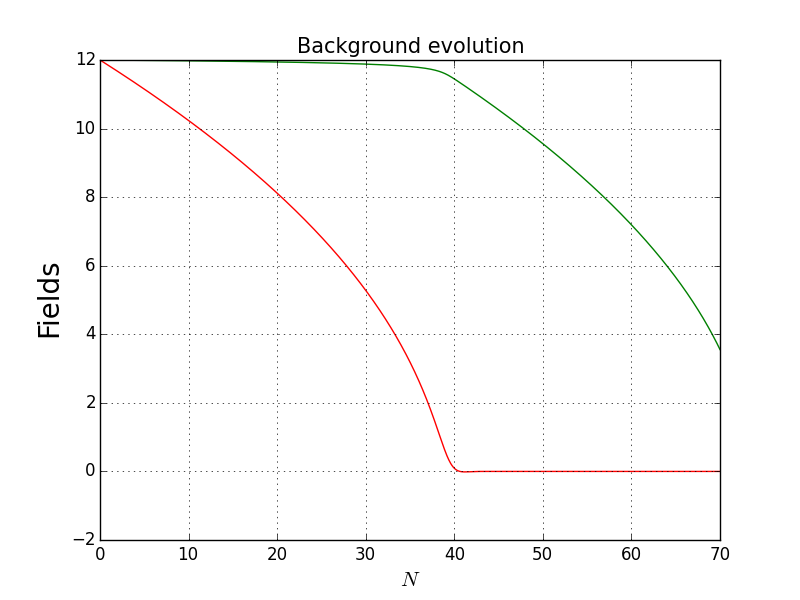
\includegraphics[width=10cm]{DQ1}
\caption{\label{double1}
Background evolution for double quadratic potential}\label{shot3}
\end{figure}
\begin{figure}[H]
\centering
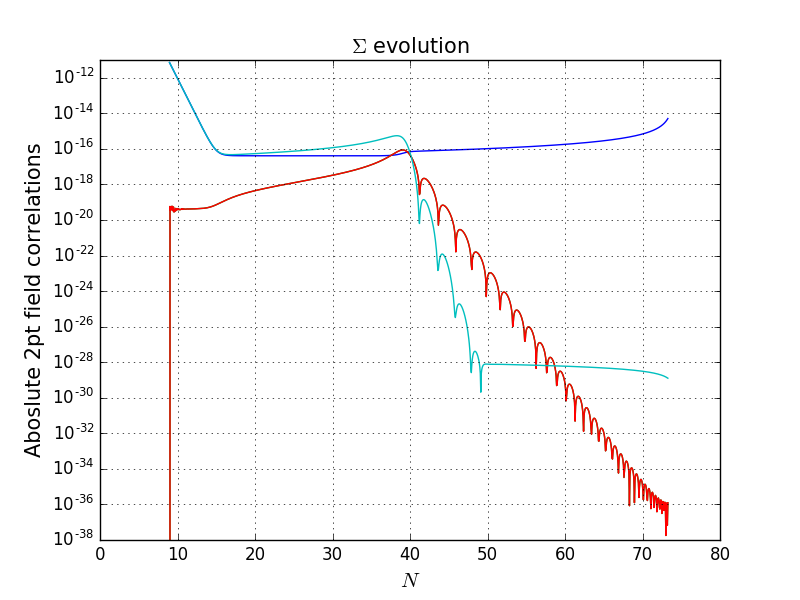
\includegraphics[width=8cm]{DQ2}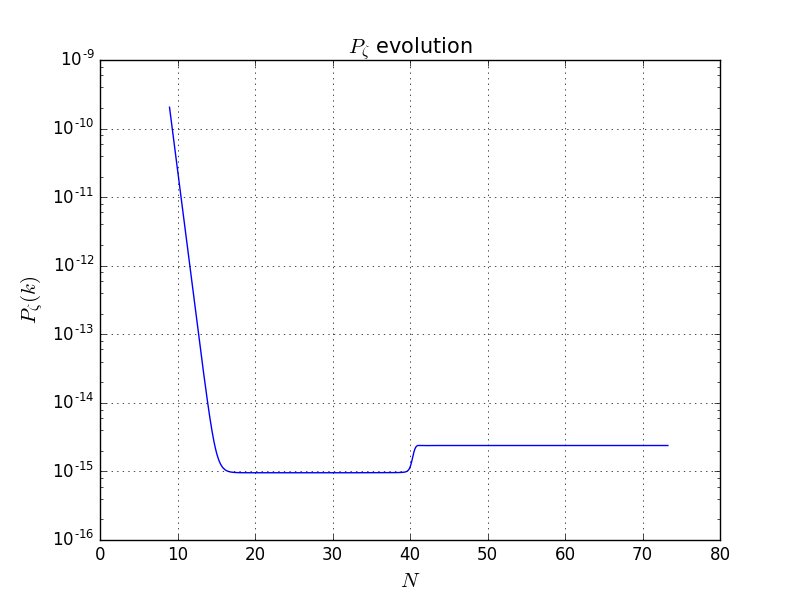
\includegraphics[width=8cm]{DQ3}\
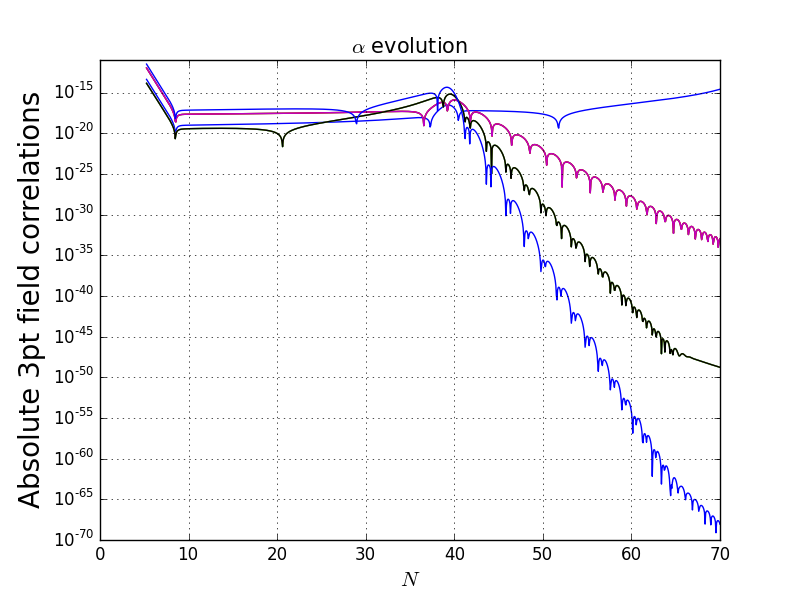
\includegraphics[width=8cm]{DQ4}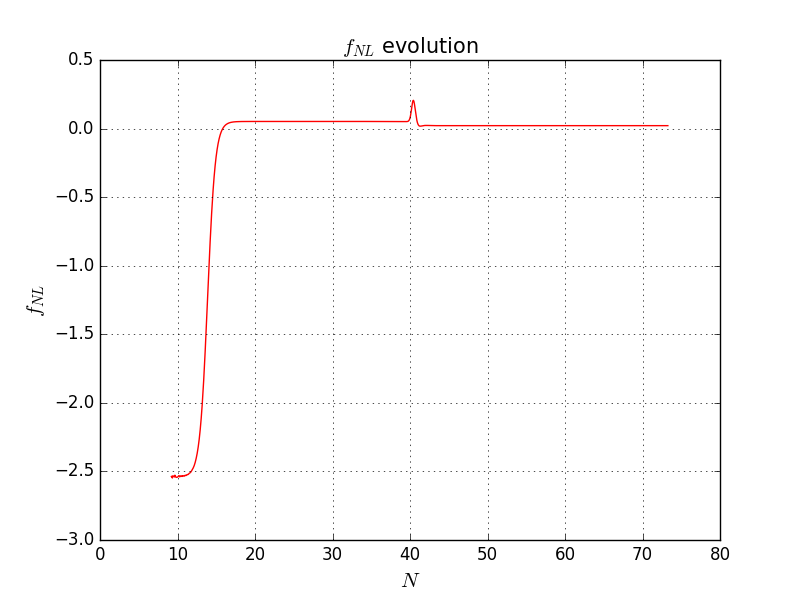
\includegraphics[width=8cm]{DQ5}\
\caption{\label{double2}
Evolution of correlations for double quadratic potential from $5$ e-folds inside the 
horizon for a Fourier mode
which crosses the horizon at $N=10$}\label{shot3}
\end{figure}

There are few things to note from this script. First we note that 
it is important that we fix our final time sensibly. If we were to fix them after the end of inflation, when the lighter field 
oscillates indefinitely about its minimum, then the code would become very slow when it evaluates the 
correlations (since the the field correlations also oscillate a lot in 
response). Next we note the use of a function within {\it PyTransScripts.py} which 
finds the k value which corresponds to an exit time of 10 e-folds after the start of the fiducial run, the {\it PyTransScripts.kexitN} 
function. This function 
uses the background trajectory and Python spline routines to find this k.
We also note that it is essential that we run the two and three point correlation evolution 
from a time the k mode of interest is deep inside the horizon, and we calculate this time 
as well as the field and field derivative values at this time 
(which are then fed into the two and three point evolution routines) using another function from the 
scripts module, the {\it PyTrans.Scripts.ICsBE} function. 
To use this function we need to specify the number of e-folds we require before horizon crossing, and here we specify $6.0$. 
It is important to point out that this function is only approximate and requires 
the background fiducial evolution which is fed into it to be finely sampled 
(10 points per e-fold is a rough guide) to be accurate 
(this is because it simply finds the value of the first $N$ 
of the background $N$ array which is before the specified number of e-folds before horizon 
crossing and returns this value and the corresponding field and field derivative fields at this time). Finally, we note 
that within {\it PyTransScripts.py} we also include the related functions  {\it kexitPhi} which finds the k value which 
crosses the horizon at a particular field value, and and {\it ICsBM} which finds initial conditions a 
fixed time before the ``massless condition" which is discussed further in section~\ref{heavy}.  These functions 
and all others in this module are detailed in Appendix 4.

Calculating the value of $n_s$ in the manner presented 
here is clearly a bad way of doing things, since it involves using only two points 
in the power spectrum to calculate a derivative, and the step between them is arbitrarily chosen, 
so it is likely to be inaccurate. 
An alternative is to calculate the power spectrum 
around a given exit time using a number of points, and to fit a spline to it and differentiate. We now generate the 
power spectrum for this model with the 
following script which fits a spline to the entire spectrum, differentiates and produces $n_s$ at every value of 
$k$ over roughly 30 e-folds, the results are plotted in Fig.~\ref{power} (the start of the file is identical to that above):
\begin{figure}[H]
\centering
\includegraphics[width=18cm]{shot6b}
\end{figure}

Next we wish to calculate the bispectrum. Here we first we calculate the bispectrum 
in the equilateral triangle configuration as a function of the $k$ value of each 
side of the triangle. Then 
we generate (and plot using a separate plots file) a slice through the bispectrum for a given 
$k_t$ as a function of the $\alpha$, $\beta$ variables defined such that $k_1 = k_t/2 - \beta  k_2/2$, 
$ k_2 = k_t/4*(1+\alpha+\beta)$ and $k3 = k_t/4*(1-\alpha+\beta)$. 
We use two separate scripts for each of these tasks (and the plots file) which are pasted below, 
both use MPI to speed 
things up, they should be called 
using the command ``/usr/local/bin/mpiexec', '-n', '10', 'python', 'MpiEqBi.py' '' 
 (for the equilateral run, where the first part 
should be replaced 
with your location of mpiexec if different, and 10 replaced by the number of processes one desires to call): 
\begin{figure}[H]
\centering
\includegraphics[width=18cm]{shot7}
\end{figure}

\begin{figure}[H]
\centering
\includegraphics[width=18cm]{shot8b}
\end{figure}

\begin{figure}
\centering
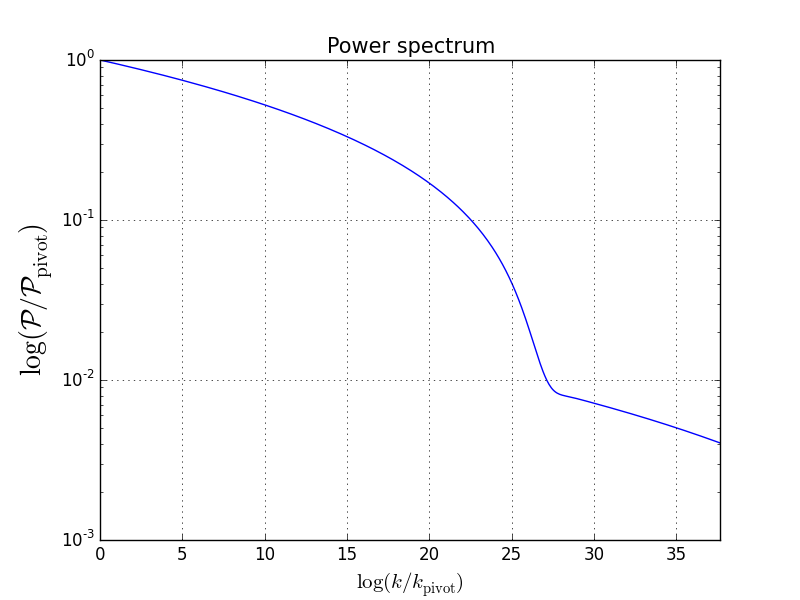
\includegraphics[width=8cm]{Pz}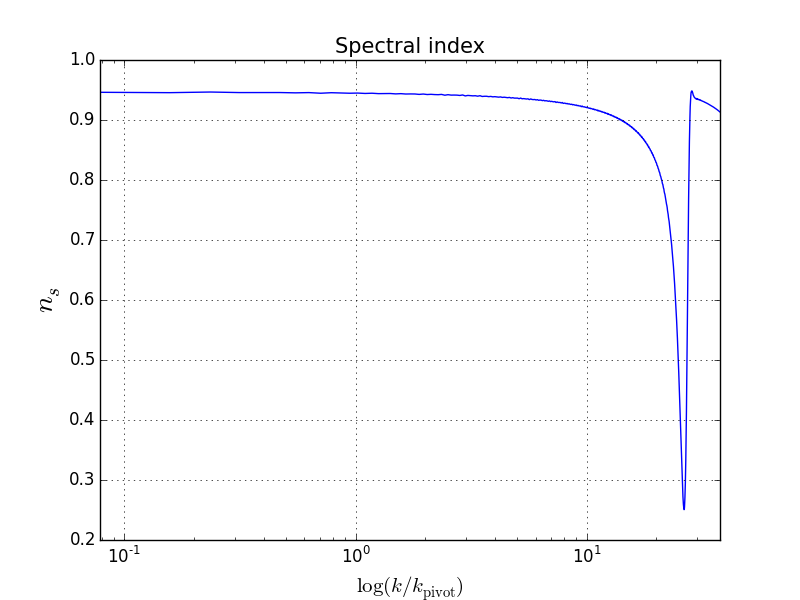
\includegraphics[width=8cm]{ns}
\caption{The power spectrum and $n_s$ in the double quadratic model. \label{power}}
\end{figure}

\begin{figure}
\centering
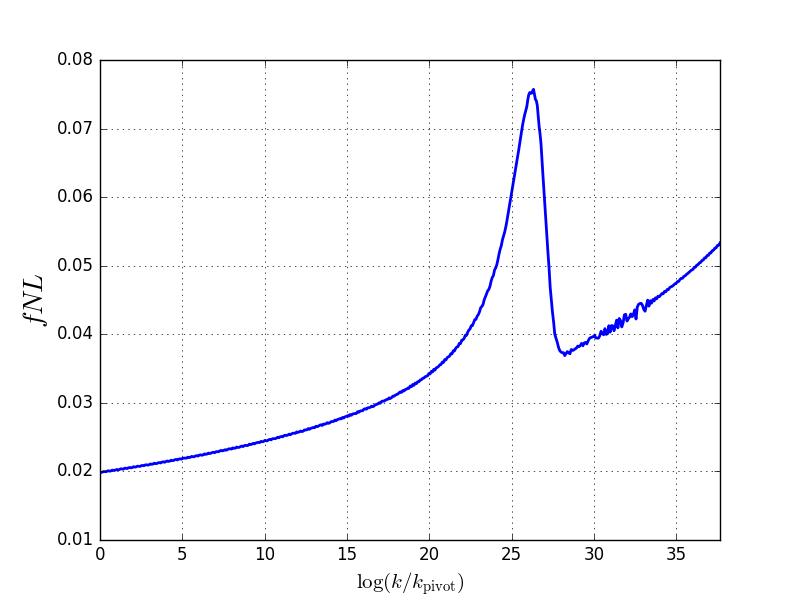
\includegraphics[width=8cm]{BiEq}
\caption{The reduced bispectrum in equilateral configurations for the double quadratic potential.\label{eqi}}
\end{figure}

\begin{figure}
\centering
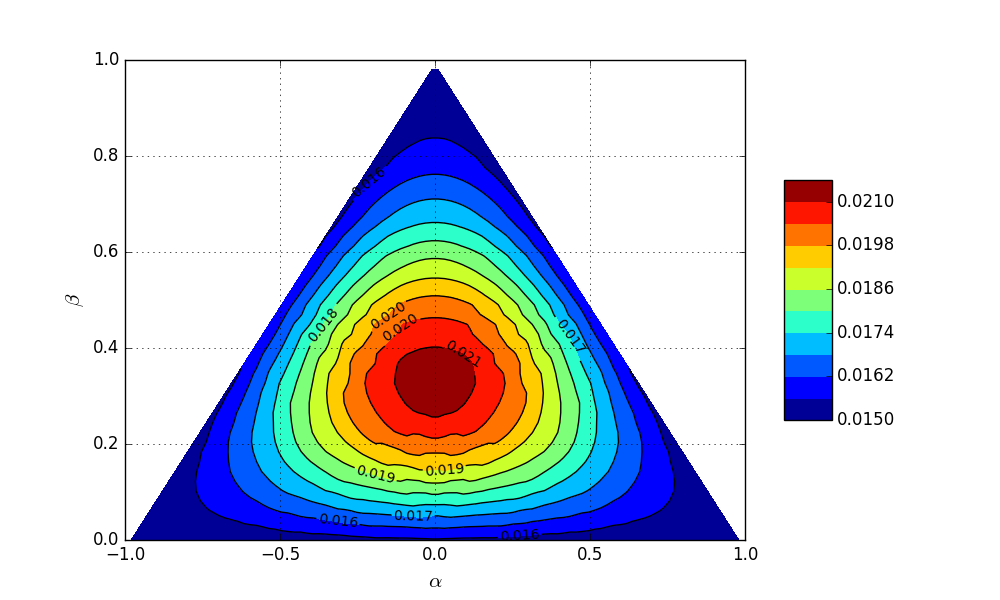
\includegraphics[width=9cm]{alpBetEq3} \hspace{-1cm}
\includegraphics[width=7.5cm]{alpBetMay}
\caption{A slice through the reduced bispectrum for a mode exiting after $15$ e-folds for the double quadratic potential run discussed in the text. \label{alpbet}}
\end{figure}

The results are in Figs.~\ref{eqi} and \ref{alpbet} respectively. 
Note that in all these scripts we use more functions available from the {\it PyTransScripts} module whose function 
should be self evident, and are described in full in Appendix 4.
If one didn't wish to use MPI the only change needed would be to call the function {\it alpBetSpec} rather than 
{\it alpBetSpecMpi} from the scripts module, and to remove MPI related lines and reference to 
rank etc.
When using MPI we recommend calling more processes 
that the system has cores. This is because we have not implemented sophisticated load sharing, and since 
some ranges will be faster to evaluate than others, if 
the number of processes is larger than cores, the cores that have capacity first will end up running more processes, 
sharing the load in a simple way. In this example we also save the data at the end for future use. This can be done 
simply for any numpy array, and then read back into Python easily. For reasons of simplicity and flexibility 
we leave data management up to the user, but note that Python is a powerful tool for this purpose.

Appendix 3 contains a summary of all the functions available to this module.

If we want to generate the full bispectrum we would simply loop over the {\it alpBetSpec} or {\it alpBetSpecMpi}
function for many $k_t$.

\subsection{Heavy field examples}
\label{heavy}

In the previous example both fields which played a role in the dynamics 
were light (at least at the start of the evolution). Interesting dynamics 
can also occur with a heavy field in the orthogonal direction to the direction of travel 
in field space, if 
the field trajectory curves and the heavy field effects can feed into the adiabatic 
perturbation. In this kind of example it is imperative that the initial conditions for the evolution of the two and three point functions are set when the $k^2/a^2$ term in the equation of motion for the scalar field perturbations 
dominates over the mass squared of the heavy 
field. This is a requirement for our initial conditions to be accurate as discussed in Ref~\cite{xxx}. 
There is a script in {\it PyTransScripts.py} which 
will achieve this, the {\it ICsBM} function. This finds initial conditions a user specified number of e-folds before the 
massless condition where $k^2/a^=M^2$ (where M is the largest eigenvalue of the mass matrix). 
There is also the function {\it ICs} which evaluates initial conditions using {\it ICsBE} (the before horizon exit 
function) and {\it ICsBM}, and takes the earliest one. The power spectrum and bipsectrum routines use this one for safety.

One example is the potential:
\be
V = \frac{1}{2} m^2_\phi \phi^2 + \frac{1}{2}M^2 \cos^2\left ( \frac{\Delta \theta}{2} \right) \left [\chi - (\phi - \phi_0 ) \tan \Xi \right]^2 
\ee
where 
\be
\Xi = \frac{\Delta \Theta}{\phi} \arctan[s (\phi - \phi_0)]
\ee
which is from Ref.~\cite{Gao:2013ota} and is in the {it LH/} folder in {\it Examples/} with some 
simple scripts to those discussed above for the double quadratic potential for users to play with. 
This example is also discussed at length in Ref.~\ref{xxx}.


\subsection{Further examples}
\label{other}

Also in the {\it Examples/} folder is another light field example with more interesting dynamics than the double quadratic 
example which we refer to as the axion quartic model, again this is accompanied 
with scripts and plots for users to explore -- this 
example was also discussed in Ref.~\ref{xxx}. This is in the {\it QuadAx} folder, and has the potential
\be
V = \frac{1}{4} \lambda \phi^4 + \Lambda^4 \left ( 1 - \cos \left ( \frac{2\pi \chi}{f} \right) \right )\,.
\ee
%A further heavy field example with potential
%\be
%V = V_0 \left (10 - \sqrt {2 \epsilon_s} \arctan \left ( \frac{\phi}{\chi} \right ) +    \frac{1}{2} m_\chi^2 
%\left ( \sqrt {\left (\chi^2 + \phi^2 \right )} - 2 \right )^2 \right)
%\ee
%is in the curve folder which was intended to illustrate gelaton-type behaviour, 

Finally in the {\it Examples/} folder and discussed in  Ref.~\ref{xxx} is a single field example with a step in the potential:
\be
V = \frac{1}{2} m^2 \phi^2 \left (1+c \tanh\left(\frac{\phi-\phi_0}{d} \right)\right)
\ee
which is in the folder {\it SingleField/} and was discussed in Refs.~\ref{Chen:2006xjb,Chen:2008wn}.


\section{Things that can go wrong}

While using the PyTransport package some issues have presented themselves which it might be useful 
for new users to know about. Many more have been ironed out, but it is neither practical nor desirable to make the code 
fully immune to misuse. We have tired to balance robustness against simplicity and ease of use, but 
below we detail a few common problems we have faced. 


\subsection{Potential computation fails}

This is the most severe bug/problem we have found, but also the least common. 

The function {\it PyTransScripts.potential(V)} takes a potential V written in the sympy format and 
calculates and then simplifies its derivatives using the function {\it sympy.simplify}. As discussed at 
this \href{http://docs.sympy.org/latest/tutorial/simplification.html}{reference}\footnote{http://docs.sympy.org/latest/tutorial/simplification.html}, however, this is not always 
the best way to simplify an expression and can also take some time to complete the simplification 
for complicated. For example the simplification process takes a relatively long time (tens of seconds) for the LH model 
above.

A more serious problem occured when looking at the example:
\be
V = V_0 \left (10 - \sqrt {2 \epsilon_s} \arctan \left ( \frac{\phi}{\chi} \right ) +    \frac{1}{2} m_\chi^2 
\left ( \sqrt {\left (\chi^2 + \phi^2 \right )} - 2 \right )^2 \right)
\ee
which represents a semi-circle curve with heavy orthogonal direction.
For this example, there appears to be a 
{\t SimPy.simplify} bug which made it crash with 
the potential written in the form given above. The origin of the problem appears to be for cross derivatives 
of the term 
in brackets which is 
multiplied by $m_\chi^2$. The problem can be worked around either by expanding this bracket manually
or by changing the {\t PyTransSetup.potential} function 
removing the use of the simplify function. There is therefore no barrier to studying this potential, but 
uncommon errors such as this are something users might need to watch out for. 

\subsection{Make sure latest module version is imported}

A more common problem is that if we wish to update a complied PyTrans*** module, for 
example after altering the tolerances, then after recompiling the module we need to 
ensure the new module is imported. The only reliable way to do this seems to be to restart or open 
a new Python session
 and then use the import command. If working in the Canopy editor, for example, this can be achieved by selecting 
 ``restart kernel" from the ``run" menu. 

\subsection{Selecting the absolute and relative tolerances}

The evolution of the three point function in particular is a numerically intensive task, and requires high numerical 
accuracy. The question arises how low (the lower the higher the accuracy) do we need to set numerical 
tolerances. This question can't be answered absolutely, and must be dealt with on a model by model basis. Models 
with finer features in the potential, or in which the excitation of the two and three point function 
occurs on sub-horizon scales will require higher tolerances. Models which produce a small signature may also need 
higher accuracy to resolve the true answer from noise than models which produce a large bispectrum. For example noise 
in the reduced bispectrum at {\cal O} $10^{-2} $ is probably acceptable for models which produce $f_{\rm NL}$ {\cal O} $1$ or higher, but 
probably not if the signal is {\cal O} $10^{-1} $.

Convergence is the key criterion in selecting tolerances. If one calculates the evolution of the three-point 
function of $\zeta$ for a example run with a given potential, reduce the tolerances and run again, without the answer 
changing in any significant manner, then the tolerances are likely to be sufficient.  As a rule of thumb 
$10^-8$ for the absolute tolorance and $10^-8$ for the relative tolerance is almost always sufficient. 
However, some examples do require lower values. As the values 
are lowered,  the code takes longer to run and eventually will fail (described below). Therefore, 
there is significant benefit for picking a required accuracy which is sufficient for the task, but not one which is too 
stringent. Those with experience of solving ODEs numerically will be familiar with this problem, which is of course 
more general than the integration at hand.

\subsection{Integration stalling or failing} 

The consequences of picking a tolerance that is too demanding can be that the integrator will not finish. 
But this can also be a consequence of setting silly initial conditions or parameter choices. It is always a good idea 
once you begin with a new model of inflation to build up gradually. First integrate the background. Even here it 
is possible for the code to take a long time. If for example the final time is after the end of inflation the code will 
try and  track all the oscillations of the field. As these increase exponentially with e-fold it 
can be very time consuming. 
Once the background is giving sensible output, move onto integrating the correlations, 
initially just for a 
single k value of the power spectrum or single triangle of the bispectrum. If 
everything looks good then run over many values to calculate the power or bi-spectrum. If you feel you are waiting too long try just asking 
the code to evolve 
a short e-folding time (.1 say). Typically a single triangle of the bispectrum evaluated before the end of 
inflation will take 
from between a fraction of a second to half a minute to run, depending on the required accuracy and 
the number of e-folds 
of sub-horizon evolution. If its still not running double check you are working 
with the correct potential for your initial conditions and parameter choices.

\subsection{Integration failing}

If the code can't reach the accuracy demanded by the user the rkf45 routine will stop running and issue an error 
message that the required accuracy couldn't be reached. 

\subsection{Not enough efolds before horizon exit}

A requirement that needs to be met in order to get accurate power spectra and bispectrum is that all the k values 
involved in, for example, a given correlation must be sufficiently deep inside the horizon initially for the initial conditions to be accurate. Since the functions which find the initial conditions for the two and three point evolutions take a background 
trajectory as their input, this trajectory must have enough e-folds prior to the exit of the k values of 
interest so that the correct initial conditions can be found. 

Moreover we must choose how many e-folds these k values stay sub-horizon for. As described above we can either 
measure backwards from horizon crossing itself or from the massless condition (only suitable for models with heavy fields) or pick 
the earliest of the two conditions. 
Normally 4-5 e-fold from these points is about right. But as with the 
setting of tolerances the only way to tell for sure is to demand convergence. Too little run in 
time leads to spurious oscillations in the spectra.

\subsection{Not enough efolds after horizon exit}

For single field models or effective single field models such as models with orthogonal heavy fields, the correlations of 
$\zeta$ become conserved after horizon crossing. Likewise if there are multiple additional light 
fields which then decay leading to 
adiabatic evolution $\zeta$ also becomes conserved. In the former case conservation only 
occurs a few e-folds after 
horizon crossing and in the latter the process also takes a few e-folds to complete. 
We must ensure, therefore, that the statistics are 
evaluated at a time when $\zeta$ has become conserved if that is what is intended, and so our evaluation time 
must be sufficiently far after horizon crossing or field decay.

\subsection{Computer crashes and data loss}

The { PyTrans***} compiled module returns data in memory to Python. Moreover, the functions provided 
to calculate power spectra and bispectra which loop over the complied module also return 
arrays of data in memory to the calling process. This is true even for the MPI functions. If anything goes wrong before these functions complete the data is lost. For example if the computer crashes, or if using distributed computing any 
one of process crashes, all the data is lost. These modules can be easily edited by users to instead write data to disk 
periodically. We have not 
included this functionality to avoid overly complicated functions, and in any case, we anticipate that 
different users will have different needs, but it is an issue to look out for.


\section{Summary}

We have presented the PyTransport package for the calculations of inflationary spectra. This package 
compliments and extends currently available tools, and is also complimentary to two related packages 
mTransport \cite{Dias:2015rca} and CppTransport \cite{xxx,xxx2}  all described at this \href{https://transportmethod.com}{website}\footnote{https://transportmethod.com}.

Through use of a detailed example we have shown how PyTransport can be used in practice. We have summarised the structure of 
the code, with some more details provided in the appendices, for those wishing to 
modify or extend the package. 

%\acknowledgement  
\begin{acknowledgments}
DJM is supported by a Royal Society University research fellowship. This work would not have been possible without 
the related collaboration with David Seery, Mafalda Dias and Jonathan Frazer. We also thank John Ronayne for vital feedback and ongoing work on future releases.
\end{acknowledgments}


\section*{Appendix 1:  Base code description}
We now give a brief description of the \CC \S  code which is the core of PyTransport. 

The folder  {\it TransportDist/PyTransport/CppTrans/} contains the base \CC \S code which the complied Python module uses.
There are  five header files in this directory. The biggest is the {\it model.h} file. This contains the model class, which 
defines the properties of an inflationary model. It contains member functions which allow the calculation of important 
properties of the inflationary model, from simple objects such as the value of the Hubble rate, to more complex ones such 
as the 
$A$, $B$, $C$ tensors which define the third order action, as discussed in Ref.~\cite{xxx}. It also calculats the ``N" tensors 
mentioned in the main text
which determine how field fluctuations are related to $\zeta$. 
The equations are motion are written in terms of $u$ tensors (see section~5 of Ref.~\ref{xxx}) which define the 
equations of motion. As noted in the main text 
we rescale the field velocity perturbation using the {\it scale} function contained in the model class. This rescaling alters the 
member classes which calculate $u_2$ and $u_3$. The output of these function is also divided by the Hubble rate, changing the 
time variable from cosmic time to $N$, e-fold time.  The scaling we choose essentially means the initial conditions for 
correlations of the velocity perturbations
are of the same order of magnitude as correlations of field perturbations, helping performance of the integrator. 
The member function that returns the ``N'' tensors is also rescaled to compensate for this change.

The {\it moments.h} file contains classes which define properties of the two and three point functions of field perturbations. 
This class is not extensively used by the Python code, but the constructor of these classes allows an instance of the 
two/three-point function to be created containing the values these objects take deep inside the horizon -- ie the initial 
conditions needed by the code. 
Once again these initial conditions are rescaled using the {\it scale} member function of the model class so that the initial 
conditions match the evolved 
correlations.

The {\it potential.h} file contains a class which defines the properties of the potential, and importantly has member functions which provide the derivatives of V. There is no barrier to changing this file by hand for a new potential. But the directory also contains {\it potentialProto.h}, which is a file that contains the skeleton of the potential.h file, and is used to automatically generate a potential.h file by the {\it PyTransSetup.potential()} function, detailed in Appendix 1.

The the {\it evolve.h} file contains functions which define the evolution equations for three systems (background only, two point 
coupled to background, and three point coupled to two point coupled to background -- the system of equations of the latter two are given 
in Eqs.~(5.5) and (5.16) of Ref.~\cite{xxx}) in the form needed 
by the rk45 ODE stepper we use. These equations use the ``u" tensors which are also described in 
section~5 of Ref.~\cite{xxx} and 
which are calculated by the {\it model.h} class.  

Finally there is a folder called rk45 stepper
which contains the files the ODE solver routine we use.


\section*{Appendix 2: Setup functions}

The functions which are part of the { PyTransSetup} modules.

\begin{itemize}
\item    {\it \bf PyTransSetup.directory()} takes no arguments and automatically edits the \CC \S files ({\it potential.h}, {\it model.h}, {\it moments.h}) so that they know about their absolute location in the file system. A user shouldn't need to call this function themselves, it is called by the compile functions below.
\item    {\it \bf PyTransSetup.pathSet()} takes no arguments and adds the location of {\it PyTrans} compiled module to the Python path. This function was called in the examples above.
\item    {\it \bf PyTransSetup.tol(rtol, atol)} takes a relative tolorance and absolute tolorance provided by the user and edits the \CC \S code such that these are the ones compiled into the compiled Python module. If not run before compiling the values last used remain in the \CC \S code. This routine is used in the examples above.
\item    {\it \bf PyTransSetup.potential(V,nF,nP)} takes a expression in SymPy format (V), which is a function of two SymPy arrays p and f, and integers nF and nP which are of length of the arrays p and f. The function then writes this potential and its derivates into the potential.h file (using the {\it potentialProto.h} file).

\item    {\it \bf PyTransSetup.compile()}  takes no arguments and complies the \CC \S  code into the Python module 
{\it PyTrans} as discussed in the text. The module is placed in the folder {\it PyTransport/PyTrans/lib/Python/}.
\item {\it \bf PyTransSetup.compileName(Name)} takes the argument name and complies the \CC \S  code into a Python module called `{\it PyTransName}. The module is placed in the folder {\it PyTransport/PyTrans/lib/Python/}.
\item {\it \bf PyTransSetup.deleteModule(Name)} takes the argument name and deletes the compiled module {\it PyTransName}.
\end{itemize}

\section*{Appendix 3: Compiled module }

The functions which are part of the complied PyTrans module are detailed below. 

These functions essentially use the \CC \S  code in the {\it CppTrans/} folder to perform various tasks. 
The code for the functions can be found in the file {\it PyTrans/PyTrans.cpp} file. This code 
should be clear to those who are familiar with \CC. The only elements which might unfamiliar are those which 
convert the \CC \S  arrays to numpy arrays (at input and output), and the part of the file which defines how distutils 
is to turn the code into a Python module. A guide to creating compiled Python modules which we followed can be found \href{http://www.tutorialspoint.com/python/python_further_extensions.htm}{at this tutorial page}\footnote{\rm http://www.tutorialspoint.com/python/python\_further\_extensions.htm}.

One other point to note is that the code which defined the functions which evolve correlations invoke a scaling (the kscale variable in the code), 
which means the integrator performs well for very different input values of the wave numbers. The rescaling is then reversed 
for output values which are returned to code calling the function.

Note the *** (Name) label needs to be added to the functions below if the module has been given a name, as described in the main text.

\begin{itemize}
\item    {\it \bf PyTrans.nF()} takes no arguments and returns the number of fields present in the model.  
\item    {\it \bf PyTrans.nP()} takes no arguments and returns the number of parameters used to define the model.
\item    {\it \bf PyTrans.V(fields, params)} takes a numpy array of length nF (the number of fields) containing a set 
    of field values, and a numpy array of length nP (the number of parameters) containing parameter values  and returns the value of the potential.
\item  {\it \bf PyTrans.dV(fields, params)} takes a numpy array of length nF (the number of fields) containing a set 
    of field values, and a numpy array of length nP (the number of parameters) containing parameter values and returns a numpy array of length nF, which contains the first derivative of the potential.
\item  {\it \bf PyTrans.dVV(fields, params)} takes a numpy array of length nF (the number of fields) containing a set 
    of field values, and a numpy array of length nP (the number of parameters) containing parameter values 
    and returns a two dimensional 
    numpy array of size nF by nF, which   
    contains the second derivative of the potential
\item  {\it \bf PyTrans.H(fields-dotfields, params)} takes an numpy array of length 2 nF (twice the number of 
    fields) containing a set of field values followed by the field's velocities in cosmic time 
    (field derivative wrt cosmic time), and an array of length nP  containing parameter values 
    and returns the value of the Hubble rate.
\item  {\it \bf PyTrans.backEvolve(Narray, fields-dotfields,params)} takes a numpy array of times in efolds (N) 
    at which we want to know the background value of the fields and field derivatives. 
    This must start with the initial N we wish to evolve the system from, and finish with the 
    final N. It also takes the initial conditions at the initial N (field values followed by 
    field velocities) as a numpy array, as well as 
    a numpy array of length nP  containing parameter values.  It returns a two dimensional numpy array. 
    This file contains the fields, and field velocities at the times requested by 
    Narray. The format is 1 + 2nF columns, with the first column the times (Narray), the next 
    columns are the field values and field velocity values at those times. 
\item  {\it \bf PyTrans.sigEvolve(Narray, k, fields-dotfields, params, full)} takes a numpy array of times in efolds (N) 
    at which we want to know the value of the two point function of inflationary perturbations. 
    This must start with the initial N we wish to evolve the system from, and finish with the 
    final N. It also takes a Fourier mode value 
    (k), and the initial conditions of the background cosmology at the initial time, the parameters of the system, 
    and an integer "full" set to 0 or 1 
    (if another value it defaults to 1). The function returns a two dimensional array 
     the first column of which contains the times (Narray), and the next 2nF  columns contains 
     the fields, and field velocities at the time steps requested. If full=0 the next column contains the power spectrum 
     of zeta, and this is the final column 
     (there are therefore 1+2nF + 1 columns in total).
     If full = 1 then there is in addition 2 nF * 2 nF columns which contain the  real parts of the matrix $\Sigma_r^{ab}$ (the power 
     spectrum and cross correlations of the fields and field velocities). 
  	The convention is that the element $\Sigma_r^{ab}$ corresponds to the [1 + 2nF + 1 + a+ 
    2nF x (b-1)]th column of the array. 
\item  {\it \bf PyTrans.alpEvolve(Narray, k1, k2, k3, fields-dotfields, params, full)} takes a numpy array of times in efolds (N) 
    at which we want to know the value of the three point function of inflationary perturbations. 
    This must start with the initial N we wish to evolve the system from, and finish with the 
    final N. It also takes three Fourier mode values 
    (k1, k2, k3), and the initial conditions at the initial time, the parameters of the system, 
    and an integer ``ful'' set to 0 or 1 
    (if another value it defaults to 1). 
    The function returns a two dimensional array 
     the first column of which contains the times (Narray), and the next 2nF  columns contains 
     the fields, and field velocities at the time steps requested (the background cosmology).
    If full=0 the next four columns contains the the power spectrum of zeta 
     for each of the three k values input, and the value of the 
     bispectrum of zeta for these k values. A total of [1+ 2nF + 4] columns. If full =1, there are 
     an additional 6 * nF*nF + nF*nF*nF columns. The first 2nF * 2nF of these contain the real 
    parts of $\Sigma^{ab}(k_1)$ in the same numbering convention as above. Then the real part of 
    $\Sigma^{ab}(k_2)$ and then the real parts of $\Sigma^{ab}(k_3)$, the following 3 * 2nF * 2nF columns are 
    the imaginary parts of the $\Sigma^{ab}(k_1)$, $\Sigma^{ab}(k_2)$ and $\Sigma^{ab}(k_3)$ matrices. So for 
    example if one wanted access to the $\Sigma_i^{ab}(k_2)$ element that would be the 
    [1 + 2nF + 4 * 2nF * 2nF + a + 2nF * (b-1)]th column of the file. The final 
    2nF * 2nF * 2nF columns of this file correspond to the $B^{abc}(k_1,k_2,k_3)$ matrix, such that     
    the corresponding columns would be the [1 + 2nF + 6 * 2nF * 2nF + a + 2nF * (b-1) + 
    2nF * 2nF * 2nF * (c-1)]th columns. 
\end{itemize}

\section*{Appendix 4: Python Scripts}

The functions which are part of the PyTransScripts modules are detailed below. The code 
which provides these scripts in the {\it PyTransScripts.py} file should be clear to those familiar with Python. The scripts are  
simply an indication of what is possible, and it is intended that users will modify them for their own purposes or 
write their own, as well as using the ones provided. 

\begin{itemize}
\item   { \it \bf PyTransScripts.ICsBE(NBExit,k, back, params, PyT)} takes in the number of e-folds before hoirzon exit of a scale k at 
which initial conditions for the evolution of correlations are to be set, the scale k itself, a background run of the cosmology (returned from PyTrans.backEvolve), the parameters of the model, and the PyTrans module being used. It returns the starting number of efolds which are at least NBExit before exit, as measured with respect to the background trajectory, back, and an array with the initial value of the fields and field derivatives at this starting time. This scripts simply runs through the elements of back to find the first one before the exit time minus NBExit. As such 
it requires back to have enough entries for the result to be, 
useful (roughly 10 per e-fold is fine). 

\item { \it \bf PyTransScripts.ICsBM(NBMassless,k, back, params, PyT)} works like PyTransScripts.ICsBM, but instead of calculating initial conditions before 
exit time, it evaluates the time when $k^2/a^2 = M^2$ where $M$ is the largest eigenvalue of the mass matrix of the potential (we call this the massless condition), and returns conditions 
more than NBExit before that time. This is useful for example with a heavy field, for which we need to ensure the approximation we use to 
fix initial conditions is accurate (which required $k^2/a^2 \gg M^2$).

\item { \it \bf PyTransScripts.ICsBM(NB,k, back, params, PyT)}  takes the same arguments as the two previous 
functions and calls each in turn, then output the number of e-folds and the fields and field derivatives at the earliest time of the two. 
This is so that the start time can be set to either NB before exit or NB before the massless condition, whichever  is earlier.

\item { \it \bf PyTransScripts.kexitN(Nexit, back, params, PyT)} takes an exit time in e-folds, a background evolution which runs though this time,  
a set of parameters and the PyTrans module being used, and returns the k mode that exited at the time Nexit. This routine uses NumPy spline 
routines to fine value of k at the exit time.

\item { \it \bf PyTransScripts.kexitPhi(PhiExit, n, back, params, PyT)} takes an exit value of one of the fields, and a number indicating one of the fields (in range from 1 to nF), a background evolution which runs through this field value,  
a set of parameters and the PyTrans module being used, and returns the k mode that exited at the that field value. This routine uses NumPy spline routines to find the right k.

\item { \it \bf PyTransScripts.pSpectra(kA, back, params, NB, PyT)}: takes a numpy array specifying  a range of k, a background evolution, a set of parameters, a number of e-folds (before massless or before exit whichever is earlier) and the PyTrans module being used, and returns two numpy arrays. The first has the corresponding values of $P_\zeta$ (to the input array of k) at the end of the evolution, and the second the times taken to perform the integration for each element.

\item { \it \bf PyTransScripts.pSpecMpi(kA, back, params, NB, PyT)}: does the same as the function above but spreads the calculation across as many process as are active using mpi4py. The script which contains this function should be called using the the command ``mpiexec -n N python Script.py", where N is the number of processes to be opened. The length of kA must be divisible by N. We recommend calling at least twice as many processes as cores are available so that cores that run processes which finish first don't simply remain idle.  The function returns the two numpy arrays to the process with rank 0. Empty arrays are returned to the other processes. 


\item { \it \bf PyTransScripts.eqSpectra(kA, back, params, NB, PyT)}: takes in the same information as the function above, and returns three arrays. The first hast the corresponding values of $P_\zeta$, the second the corresponding values of $B_\zeta$ in the equilateral configuration ($k1=k2=k3=k$) at the end of the evolution, and the final hte times taken to perform the integration for each element.


\item { \it \bf PyTransScripts.eqSpecMpi(kA, back, params, NB, PyT)}: does the same as the function above but spreads the calculation across as many process as are active using mpi4py. The script which contains this function should be called using the the command ``mpiexec -n N python Script.py", where N is the number of processes to be opened. The length of kA must be divisible by N. We recommend calling at least twice as many processes as cores are available so that cores that run processes which finish first don't simply remain idle.  The function returns the three numpy arrays to the process with rank 0. Empty arrays are returned to the other processes. 


\item { \it \bf PyTransScripts.alpBetSpectra(kt,alpha, beta, back, params, NB, nsnaps, PyT)}: takes in a value of kt, and two arrays defining a range of values of alpha and beta, as well as a background evolution, set of parameters and a number of e-folds before horizon exit or the massless condition is met. It also takes an integer nsnaps, and the PyTrans module being used. nsnaps  tells the code at how many different times to provide output. It outputs six arrays. The first output array is the $B_\zeta$ at values corresponding to the values in the input arrays alpha and beta. The second is $P_zeta(k_1)$ for this values, the next $P_\zeta(k_2)$ and the next $P_\zeta(k_3)$. If nsnaps is 0 or 1, the third dimension of these arrays is only 1 element long, and the values returned correspond to those at the end of the evolution. If it is greater than one values at evenly space times from 2 e-folds inside the horizon until the end of the evolution are 
returned. This allows us to see how a slice through bispectrum evolves with time if we wish. The fifth array is two dimensional 
and corresponds to the times taken to perform the integrations associated with every combination of alpha and beta. The last array is the 
times of the nsnaps.

\item { \it \bf PyTransScripts.alpBetMpi(kt,alpha, beta, back, params, NB, nsnaps, PyT)}: does the same as the function above but spreads the calculation across as many process as are active using mpi4py. The script which contains this function should be called using the the command ``mpiexec -n N python Script.py", where N is the number of processes to be opened. The length of alpha must be divisible by N. We recommend calling at least twice as many processes as cores are available so that cores that run processes which finish first don't simply remain idle.  The function returns the five numpy arrays to the process with rank 0. Empty arrays are returned to the other processes. 

\end{itemize}

\bibliography{paper}

%%%%%%%%%%%%%%%%%%%%%%%%%%%%%%%%%%%%%%%%%%%%%%%%%%%%%%%%%%%%%%%%%%%%%%

\end{document}